\documentclass{revtex4-1}
\usepackage{amsmath, latexsym, braket, amsfonts, url, bbold, amssymb, graphicx}
\setcounter{secnumdepth}{5}

\begin{document}

% Top Matter
\title{Lanczos Bound-state Calculation Code}
\author{Joshua T. Cantin}
%\address{Department of Chemistry, University of Waterloo, Waterloo, Ontario N2L 3G1, Canada}
\date{\today}

\maketitle

\section{Introduction}\label{S:intro}
This document contains both documentation concerning the Lanczos Bound-state Calculation Code as well as information about the underlying theory.

\section{Theory}\label{S:theory}
It should be noted that it is possible that one could define a combined basis $\ket{\gamma}$ that represents $\ket{\gamma}=\ket{\alpha\beta}=\ket{\alpha}\ket{\beta}$ such that $\gamma[\alpha,\beta]$ in a similar manner to that done with $n[l,m]$ for the $\ket{n}=\ket{lm}$ Tesseral Harmonic basis.

We also may want to test out a specialized code (either in terms of type of rotor or the spin isomers) versus a generalized code (use the symmetrizing operator to select out the even and odd states?) and see which is computationally more efficient.

The Colbert-Miller Formulae will be used for the translational basis and the Wigner functions could possibly be used for the Asymmetric Top ($e^{im\phi}d^{J}_{MK}(\theta)e^{ik\chi}$).
\subsection{Hamiltonian}\label{S:Hamilton}
It should be noted that one may be able to define a symmetrizing operator that will allow one to select out the ortho, para or spinless states from the Hamiltonian when calculating the Krylov Subspace. The operator would act as follows
\begin{align*}
w &= \hat{S}\hat{H}v \\
w_{para} &= \hat{S}_{even}\hat{H}v \\
w_{ortho} &= \hat{S}_{odd}\hat{H}v \\
w_{spinless} &= \hat{S}_{all}\hat{H}v \\
\end{align*}
\subsubsection{Linear Rotor}\label{S:LinRotH}
The Hamiltonian for a Cartesian grid for the centre of mass position and $\theta$ and $\phi$ for the orientation is as follows:
\begin{equation}
\widehat{H}_{zxy\theta\phi} = \widehat{T}_{x} + \widehat{T}_{y} + \widehat{T}_{z} + \widehat{T}_{rot} + \widehat{V}_{xyz\theta\phi} 
\end{equation}
Now, the discrete variable representation (DVR) presented by Colbert and Miller in their 1992 paper will be used for the Cartesian grid. Specifically, the DVR for a variable that varies from $-\infty$ to $\infty$ will be used, but truncated to the box size. This DVR will behave as if the system is suspended in empty space, rather than having an infinite potential at the boundaries (i.e. particle in a box), which a DVR designed for a finite grid would represent.
The grid points are as follows:
\begin{equation}
x_{i} = i\Delta x, \text{ where } i = 0, \pm 1, \pm 2, ..., \pm \infty
\end{equation}
The corresponding basis functions are:
\begin{equation}
\braket{x|x_{i}} = \frac{\sin \left(\frac{\pi(x-x_{i})}{\Delta x}\right)}{\pi(x-x_{i})}
\end{equation}
The grid is set such that $\braket{x|x_{i}}$ is zero for all $x_{i}\neq x$. Thus, it appears that while interpolation between the grid points is possible, the value at each of the grid points is independent of all of the other grid points; I believe that this simplifies the equations and the subsequent diagonalization of the Hamiltonian. The kinetic energy operator is then expressed as 
\begin{equation}
\braket{x_{i}|\widehat{T}_{x}|x_{i'}}=\widehat{T}_{x_{i,i'}}=\frac{\hbar^{2}}{2m\Delta x^{2}} (-1)^{i-i'} \left.\begin{cases} \frac{\pi^{2}}{3}, & i=i'\\
																			    \frac{2}{(i-i')^{2}}, &i\neq i'
																			    \end{cases}\right\}
\end{equation}
where $m$ is the total mass of the linear rotor and $\Delta x$ is the grid spacing.
Note that $\widehat{T}_{x_{i,i'}}$ is diagonal in all the other grids used, whether $\ket{yz\theta\phi}$ or $\ket{yzlm}$ and that $\widehat{T}_{y_{i,i'}}$ and $\widehat{T}_{z_{i,i'}}$ are of the same form as $\widehat{T}_{x_{i,i'}}$.

For the rotation, the finite basis representation (FBR) of $\ket{lm}$ (the Tesseral Harmonics, a.k.a. the real form of the Spherical harmonics) is to be used instead of $\theta$ and $\phi$. This then makes
\begin{equation}
\widehat{H}_{zxylm} = \widehat{T}_{x} + \widehat{T}_{y} + \widehat{T}_{z} + \widehat{T}_{rot} + \widehat{V}_{xyzlm} 
\end{equation}
The rotational kinetic energy is thus
\begin{equation}
\widehat{T}_{rot} = B\hat{l}^{2}
\end{equation}
where $B$ is the rotational constant defined as
\begin{equation}
B = \frac{\hbar^{2}}{2I}
\end{equation}
with $I$ as the moment of inertia. The terms of $\widehat{T}_{rot}$ are
\begin{equation}
\braket{lm|\widehat{T}_{rot}|l'm'} = Bl(l+1)\delta_{ll'}\delta_{mm'}
\end{equation}
where $\delta_{ii'}$ is the Kronecker delta, showing that $\widehat{T}_{rot}$ is diagonal in both $l$ and $m$.

Now, the potential $\widehat{V}$ is calculated and stored in the $\ket{xyz\theta\phi}$ basis and must be converted to the $\ket{xyzlm}$ basis. First of all, the terms of $\widehat{V}$ in the $\ket{xyz\theta\phi}$ basis is
\begin{equation}
\braket{xyz\theta\phi|\widehat{V}_{xyz\theta\phi}|x'y'z'\theta'\phi'} = V(x,y,z,\theta,\phi)\delta_{xyz\theta\phi,x'y'z'\theta'\phi'}
\end{equation}
To convert from $\ket{xyz\theta\phi}$ to $\ket{xyzlm}$, one can find the elements of $\widehat{V}_{xyz\theta\phi}$ in $\ket{xyzlm}$
\begin{align}
\braket{xyzlm|\widehat{V}_{xyzlm}|x'y'z'l'm'} &= \braket{xyzlm|\widehat{V}_{xyz\theta\phi}|x'y'z'l'm'}\\
											 &= \braket{lm|\widehat{V}_{\theta\phi}(x,y,z)|l'm'}\\
											 &= \int_{\theta=0}^{\pi}\int_{\phi=0}^{2\pi}\int_{\theta=0}^{\pi}\int_{\phi=0}^{2\pi}\braket{lm|\theta\phi}\braket{\theta\phi|\widehat{V}_{\theta\phi}(x,y,z)|\theta'\phi'}\braket{\theta'\phi'|l'm'}\partial\phi \sin \theta \partial\theta \partial\phi' \sin \theta' \partial\theta'\\
											 &= \int_{\theta=0}^{\pi}\int_{\phi=0}^{2\pi}\widetilde{Y}_{lm}(\theta,\phi)V(\theta,\phi; x,y,z)\widetilde{Y}_{l'm'}(\theta,\phi)\partial\phi \sin \theta \partial\theta \\
											 \begin{split} &=\int_{\theta=0}^{\pi}\int_{p=-1}^{1}\frac{1}{\sqrt{1-p^{2}}}\lbrack\widetilde{Y}_{lm}(\theta, \cos^{-1}p)V(\theta, \cos^{-1}p; x,y,z)\widetilde{Y}_{l'm'}(\theta, \cos^{-1}p) \\&+ \widetilde{Y}_{lm}(\theta, 2\pi-\cos^{-1}p)V(\theta, 2\pi-\cos^{-1}p; x,y,z)\widetilde{Y}_{l'm'}(\theta, 2\pi-\cos^{-1}p)\rbrack \partial p \sin \theta \partial\theta \end{split}\\
											 \begin{split} &=\int_{\cos\theta=-1}^{1}\int_{p=-1}^{1}\frac{1}{\sqrt{1-p^{2}}}\lbrack\widetilde{Y}_{lm}(\theta, \cos^{-1}p)V(\theta, \cos^{-1}p; x,y,z)\widetilde{Y}_{l'm'}(\theta, \cos^{-1}p) \\&+ \widetilde{Y}_{lm}(\theta, 2\pi-\cos^{-1}p)V(\theta, 2\pi-\cos^{-1}p; x,y,z)\widetilde{Y}_{l'm'}(\theta, 2\pi-\cos^{-1}p)\rbrack \partial p  \partial (\cos \theta) \end{split}\\
											 \begin{split} &=\int_{q=-1}^{1}\int_{p=-1}^{1}\frac{1}{\sqrt{1-p^{2}}}\lbrack\widetilde{Y}_{lm}(\cos^{-1}q, \cos^{-1}p)V(\cos^{-1}q, \cos^{-1}p; x,y,z)\widetilde{Y}_{l'm'}(\cos^{-1}q, \cos^{-1}p) \\&+ \widetilde{Y}_{lm}(\cos^{-1}q, 2\pi-\cos^{-1}p)V(\cos^{-1}q, 2\pi-\cos^{-1}p; x,y,z)\widetilde{Y}_{l'm'}(\cos^{-1}q, 2\pi-\cos^{-1}p)\rbrack \partial p  \partial q \end{split}\\
											 \begin{split} &\approx\int_{q=-1}^{1}\sum_{\beta=1}^{n_{\beta}}w^{GC}_{\beta}\lbrack\widetilde{Y}_{lm}(\cos^{-1}q, \cos^{-1}p_{\beta})V(\cos^{-1}q, \cos^{-1}p_{\beta}; x,y,z)\widetilde{Y}_{l'm'}(\cos^{-1}q, \cos^{-1}p_{\beta}) \\&+ \widetilde{Y}_{lm}(\cos^{-1}q, 2\pi-\cos^{-1}p_{\beta})V(\cos^{-1}q, 2\pi-\cos^{-1}p_{\beta}; x,y,z)\widetilde{Y}_{l'm'}(\cos^{-1}q, 2\pi-\cos^{-1}p_{\beta})\rbrack \partial q \end{split}\\
											 \begin{split} &\approx\sum_{\alpha=1}^{n_{\alpha}}w^{GL}_{\alpha}\sum_{\beta=1}^{n_{\beta}}w^{GC}_{\beta}\lbrack\widetilde{Y}_{lm}(\cos^{-1}q_{\alpha}, \cos^{-1}p_{\beta})V(\cos^{-1}q_{\alpha}, \cos^{-1}p_{\beta}; x,y,z)\widetilde{Y}_{l'm'}(\cos^{-1}q_{\alpha}, \cos^{-1}p_{\beta}) \\&+ \widetilde{Y}_{lm}(\cos^{-1}q_{\alpha}, 2\pi-\cos^{-1}p_{\beta})V(\cos^{-1}q_{\alpha}, 2\pi-\cos^{-1}p_{\beta}; x,y,z)\widetilde{Y}_{l'm'}(\cos^{-1}q_{\alpha}, 2\pi-\cos^{-1}p_{\beta})\rbrack \end{split}\\
											 &=
\end{align} 
where $\widetilde{Y}_{lm}(\theta,\phi)$ are the Tesseral harmonics, $w^{GL}_{\alpha}$ and $q_{\alpha}$ are the Gauss-Legendre quadrature weights and abscissae, and $w^{GC}_{\beta}$ and $p_{\beta}$ are the Gauss-Chebyshev quadrature weights and abscissae.  NOTE: THE ABOVE THREE OR FOUR EQUATIONS HAVE DEFINITE PROBLEMS

\subsection{Basis States}\label{S:BS}
\subsubsection{Rotor Bases}\label{S:RotBS}
\paragraph{Linear Rotor}\label{S:LinRotBS}
For the linear rotor, the tesseral spherical harmonics will be used as the basis states and are defined as follows (taken from \url{http://en.wikipedia.org/wiki/Spherical_harmonics}):
\begin{align}
Y_{lm}(\theta,\phi)&=\begin{cases}\label{E:SphDefComb} 	\frac{1}{\sqrt{2}}\left(Y^{m}_{l}\left(\theta,\phi\right)+\left(-1\right)^{m}Y^{-m}_{l}\left(\theta,\phi\right)\right) &\mbox{if } m>0\\
								 	Y^{0}_{l}\left(\theta,\phi\right) &\mbox{if } m=0\\
								 	\frac{1}{i\sqrt{2}}\left(Y^{-m}_{l}\left(\theta,\phi\right)-\left(-1\right)^{m}Y^{m}_{l}\left(\theta,\phi\right)\right) &\mbox{if } m<0\\
								 	\end{cases}\\
				   &=\begin{cases}\label{E:SphDefTes} 	\sqrt{2}N_{\left(l,m\right)}P^{m}_{l}\left(\cos{\theta}\right)\cos{m\phi} &\mbox{if } m>0\\
				   					Y^{0}_{l}\left(\theta,\phi\right) &\mbox{if } m=0\\
									\sqrt{2}N_{\left(l,|m|\right)}P^{|m|}_{l}\left(\cos{\theta}\right)\sin{|m|\phi} &\mbox{if } m<0\\
				   					\end{cases}
\end{align}
where $N_{\left(l,m\right)}$ is a normalization constant and is 
\begin{equation}
N_{\left(l,m\right)}\equiv\frac{1}{\sqrt{2\pi}}\sqrt{\frac{\left(2l+1\right)}{2}\frac{\left(l-m\right)!}{\left(l+m\right)!}}
\end{equation}
Note that we incorporate the Condon-Shortley phase in $N_{\left(l,m\right)}$, so that 
\begin{equation}
N_{\left(l,m\right)}\equiv\left(-1\right)^{m}\frac{1}{\sqrt{2\pi}}\sqrt{\frac{\left(2l+1\right)}{2}\frac{\left(l-m\right)!}{\left(l+m\right)!}}
\end{equation}
$Y^{m}_{l}\left(\theta,\phi\right)$ are the Laplace Spherical Harmonics and are  
\begin{equation}
Y^{m}_{l}\left(\theta,\phi\right)=N_{\left(l,m\right)}P^{m}_{l}\left(\cos{\theta}\right)e^{im\phi}
\end{equation}

$P^{m}_{l}$ are the associated Legendre polynomials of non-negative $m$, defined as
\begin{equation}
P^{m}_{l}\left(x\right)=\left(-1\right)^{m}\left(1-x^{2}\right)^{\frac{m}{2}}\frac{d^{m}}{dx^{m}}\left(P_{l}\left(x\right)\right)
\end{equation}
where $P_{l}\left(x\right)$ are the Legendre Polynomials, expressed using Rodrigues' formula:
\begin{equation}
P_{l}\left(x\right)=\frac{1}{2^{l}l!}\frac{d^{l}}{dx^{l}}\lbrack\left(x^{2}-1\right)^{l}\rbrack
\end{equation} 

In practise, the associated Legendre Polynomials $\left(P^{m}_{l}\left(x\right)\right)$ are calculated by first calculating
\begin{equation*}
P^{l}_{l}\left(x\right)=\left(2l-1\right)P^{l-1}_{l-1}\left(x\right)\sqrt{1-x^{2}}
\end{equation*}
for $l=1 \mbox{ to } l=l_{max}$, where $P^{0}_{0}=1$.

Then, the associated Legendre Polynomials are calculated for $m=0\mbox{ to }m=l_{max}-1$ and for $l=1 \mbox{ to } l=l_{max}$ as follows
\begin{equation}
P^{l+1}_{m}\left(x\right)=\frac{\lbrack\left(2l+1\right)xP^{l}_{m}\left(x\right)-\left(l+m\right)P^{l-1}_{m}\left(x\right)\rbrack}{l-m+1}
\end{equation}
where $P^{l-1}_{m}\left(x\right)=0\mbox{ if }l-1<m$.

\subparagraph{Legendre Polynomial Recursion Relations}\label{S:LegPolyRecursive}
From Abramowitz and Stegun, pg.334, the Legendre Polynomials can be generated using the following recurrence relations, where 
\begin{align*}
&\{\nu | \nu \epsilon \mathbb{C} \}\\
&\{\mu | \mu \epsilon \mathbb{C} \}\\
&\{n | n \geq0, n \epsilon \mathbb{Z} \}\\
&\{m | m \geq0, m \epsilon \mathbb{Z} \}\\
&\{z | z \epsilon \mathbb{C} \}\\
&\{x | x \epsilon \mathbb{R} \}\\
\end{align*}
If the degree $(\nu)$ is varying,

8.5.3:
\begin{equation}
\left( \nu - \mu +1 \right)P^{\mu}_{\nu+1}\left( z \right) = (2\nu+1)zP^{\mu}_{\nu}(z)-(\nu+\mu)P^{\mu}_{\nu-1}(z)
\end{equation}

8.5.4:
\begin{equation}
(z^{2}-1) \frac{dP^{\mu}_{\nu}(z)}{dz}=\nu z P^{\mu}_{\nu}-(\nu+\mu)P^{\mu}_{\nu-1}(z)
\end{equation}

If the order $(\mu)$ is varying,

8.5.1:
\begin{equation}
P^{\mu+1}_{\nu}(z) = \sqrt{z^{2}-1} [(\nu-\mu)zP^{\mu}_{\nu}(z)-(\nu+\mu)P^{\mu}_{\nu-1}(z)]
\end{equation}

8.5.2:
\begin{equation}
(z^{2}-1)\frac{dP^{\mu}_{\nu}(z)}{dz}=(\nu+\mu)(\nu-\mu+1)\sqrt{z^{2}-1}P^{\mu-1}_{\nu}(z)-\mu z P^{\mu}_{\nu}(z)
\end{equation}

If the order $(\mu)$ and the degree $(\nu)$ are varying,

8.5.5:
\begin{equation}
P^{\mu}_{\nu+1}(z)=P^{\mu}_{\nu-1}(z)+(2\nu+1)\sqrt{z^{2}-1}P^{\mu-1}_{\nu}(z)
\end{equation}

It should also be noted that (A\&S pg.333 8.4.1 and 8.4.3)
\begin{align}
P^{0}_{0}(z) &= 1\\
P^{0}_{1}(z) &= z
\end{align}

and (A\&S pg.333 8.2.1)
\begin{equation}
P^{\mu}_{-\nu-1}(z)=P^{\mu}_{\nu}(z)
\end{equation}

For the system used here, $\mu$ can be set to $m$, $\nu$ to $n$, and $z$ to $x$, resulting in: 

If the degree $(n)$ is varying,

\begin{equation}
\left( n - m +1 \right)P^{m}_{n+1}\left( x \right) = (2n+1)xP^{m}_{n}(x)-(n+m)P^{m}_{n-1}(x)
\end{equation}

\begin{equation}
(x^{2}-1) \frac{dP^{m}_{n}(x)}{dx}=n x P^{m}_{n}-(n+m)P^{m}_{n-1}(x)
\end{equation}
and Bonnet's Recursion Formula if $m=0$ (from \url{http://en.wikipedia.org/wiki/Legendre_polynomials})
\begin{equation}
\left( n +1 \right)P_{n+1}\left( x \right) = (2n+1)xP_{n}(x)-nP_{n-1}(x)
\end{equation}
from this, the corresponding formula for the derivative is found to be (from \url{http://en.wikipedia.org/wiki/Legendre_polynomials})
\begin{equation}
(x^{2}-1) \frac{dP_{n}(x)}{dx}=n x P_{n}-nP_{n-1}(x)
\end{equation}

If the order $(m)$ is varying,

\begin{equation}
P^{m+1}_{n}(x) = \sqrt{x^{2}-1} [(n-m)xP^{m}_{n}(x)-(n+m)P^{m}_{n-1}(x)]
\end{equation}

\begin{equation}
(x^{2}-1)\frac{dP^{m}_{n}(x)}{dx}=(n+m)(n-m+1)\sqrt{x^{2}-1}P^{m-1}_{n}(x)-m x P^{m}_{n}(x)
\end{equation}

If the order $(m)$ and the degree $(n)$ are varying,

\begin{equation}
P^{m}_{n+1}(x)=P^{m}_{n-1}(x)+(2n+1)\sqrt{x^{2}-1}P^{m-1}_{n}(x)
\end{equation}

It should also be noted that (A\&S pg.333 8.4.1 and 8.4.3)
\begin{align}
P^{0}_{0}(x) &= 1\\
P^{0}_{1}(x) &= x
\end{align}


\subparagraph{Orthonormality Test of the associated Legendre Polynomials}\label{S:assocLegPolyOrthonormTest}

A numerical test of the associated Legendre Polynomials tested can be performed using their orthonormality property. The normalized associated Legendre Polynomials are defined as:
\begin{equation}
\widetilde{P}^{m}_{l}(x) = \sqrt{\frac{\left(2l+1\right)}{2}\frac{\left(l-m\right)!}{\left(l+m\right)!}} P^{m}_{l}(x)
\end{equation}
where
\begin{align*}
&\{n | n \geq0, n \epsilon \mathbb{Z} \}\\
&\{m | m \geq0, m \epsilon \mathbb{Z} \}\\
&\{x | x \epsilon \mathbb{R} \}\\
\end{align*}
and $P^{m}_{l}(x)$ are the non-normalized associated Legendre polynomials:
\begin{equation}
P^{m}_{l}\left(x\right)=\left(-1\right)^{m}\left(1-x^{2}\right)^{\frac{m}{2}}\frac{d^{m}}{dx^{m}}\left(P_{l}\left(x\right)\right)
\end{equation}
where $P_{l}\left(x\right)$ are the Legendre Polynomials, expressed using Rodrigues' formula:
\begin{equation}
P_{l}\left(x\right)=\frac{1}{2^{l}l!}\frac{d^{l}}{dx^{l}}\lbrack\left(x^{2}-1\right)^{l}\rbrack
\end{equation} 
Now, orthonormality states that, for fixed $m$,
\begin{equation}
\int_{-1}^{1} \widetilde{P}^{m}_{l}(x) \widetilde{P}^{m}_{l'}(x) dx =  \delta_{ll'}
\end{equation}
if $0 \leq m \leq l$ (taken from PN and \url{http://en.wikipedia.org/wiki/Associated_Legendre_polynomials}).
Now, based on the Gauss-Legendre Quadrature
\begin{equation}
\int_{-1}^{1} \widetilde{P}^{m}_{l}(x) \widetilde{P}^{m}_{l'}(x) dx = \sum_{\alpha=1}^{n_{\alpha}}w_{\alpha}\widetilde{P}^{m}_{l}(x_{\alpha})\widetilde{P}^{m}_{l'}(x_{\alpha}) = \delta_{ll'}
\end{equation}
where the condition $l \leq 2n-1$ is required for the relation to be exact (i.e. $R_{n}=0$), as shown. The definitions of $x_{\alpha}$ and $w_{\alpha}$ can be found in section \ref{S:gaussLegendreQuad}. If one defines a matrix,
\begin{equation}
L^{m}_{l \alpha} = \widetilde{P}^{m}_{l}(x_{\alpha})\sqrt{w_{\alpha}}
\end{equation}
then
\begin{equation}
\sum_{\alpha=1}^{n_{\alpha}}w_{\alpha}\widetilde{P}^{m}_{l}(x_{\alpha})\widetilde{P}^{m}_{l'}(x_{\alpha}) = \sum_{\alpha=1}^{n}L^{m}_{l \alpha}(L^{m}_{l' \alpha})^{\intercal} = \delta_{ll'}
\end{equation}
Also, for fixed $l$, (from \url{http://en.wikipedia.org/wiki/Associated_Legendre_polynomials})
\begin{equation}
\int_{-1}^{1} \frac{\widetilde{P}^{m}_{l}(x) \widetilde{P}^{m'}_{l}(x)}{1-x^{2}}dx = \begin{cases} 0 &\text{if } m \neq n\\
																								\frac{(l+m)!}{m(l-m)!} &\text{if } m = n \neq 0\\
																								\infty &\text{if } m = n = 0
																				   \end{cases}
\end{equation}
Thus,
\begin{equation}
L^{n\intercal}L^{m} = L^{n}L^{m\intercal} = \mathbb{1}
\end{equation}
Though I think the Chebyshev Quadrature may be needed, given the form of the integral.

Now, the $\ket{lm}$ is not a direct product of $\ket{l}$ and $\ket{m}$ (i.e. $\ket{lm} \neq \ket{l}\ket{m}$) as $l$ and $m$ are not independent quantum numbers, but $|m|\leq l, \mbox{ with the restriction that } l\geq 0$. This makes storing the $\ket{lm}$ basis in a matrix more difficult. However, this issue is at least partially alleviated by defining a new quantum number $n = l^{2}+l+m$, with $0 \leq n \leq (l_{max}^{2}+2l_{max}) =(l_{max}+1)^{2}-1$.


\subparagraph{Gauss-Legendre Quadrature}\label{S:gaussLegendreQuad}

From Abramowitz and Stegun pg.887, Section 25.4.29:

The quadrature is
\begin{equation}
\int_{-1}^{1}f(x)dx = \sum_{i=1}^{n}w_{i}f(x_{i}) + R_{n}
\end{equation}
The related polynomials for this quadrature are the Legendre Polynomials $P_{n}(x), P_{n}(1)=1$. Also,
\begin{align}
x_{i} &= i\text{th root of } P_{n}(x)\\
w_{i} &= \frac{2}{(1-x_{i}^{2})(P'_{n}(x_{i}))^{2}}\\
R_{n} &= \frac{2^{2n+1}(n!)^{4}}{(2n+1)[(2n)!]^{3}}f^{(2n)}(\xi), (-1<\xi<1)
\end{align}
It should be noted that $R_{n} = 0$ if $f(x)$ is a polynomial of degree $2n-1$ or less (as $f^{(2n)}(x) = 0$ in that case).

\subparagraph{Gauss-Chebyshev Quadrature}\label{S:gaussChebyshevQuad}

From Abramowitz and Stegun pg.889, Section 25.4.39:

The quadrature is
\begin{equation}
\int_{-1}^{1}\frac{f(x)}{\sqrt{1-x^{2}}}dx = \sum_{i=1}^{n}w_{i}f(x_{i}) + R_{n}
\end{equation}
The related orthogonal polynomials are the Chebyshev Polynomials of the First Kind:
\begin{equation}
T_{n}(x),T_{n}(1)=\frac{1}{2^{n-1}}
\end{equation}
Also,
\begin{align}
x_{i} &= \cos{\frac{(2i-1)\pi}{2n}}\\
w_{i} &= \frac{\pi}{n}\\
R_{n} &= \frac{\pi}{(2n)!2^{2n-1}}f^{(2n)}(\xi), (-1<\xi<1)
\end{align}

\subparagraph{$\ket{lm}$ Basis Notes}\label{S:lmBasis}

The $\ket{lm}$ basis size can be enumerated as follows:
\begin{align}
Count  	&= \sum_{m=-l_{max}}^{l_{max}} \sum_{l=|m|}^{l_{max}}1 \\
		&= \sum_{m=-l_{max}}^{l_{max}} (l_{max} - |m| + 1) \nonumber \\
		&= 2 \sum_{m=1}^{l_{max}}(l_{max} - m + 1) + l_{max} + 1 \nonumber \\
		&= 2l_{max}^{2} - l_{max}(l_{max} + 1) + 2l_{max} + l_{max} + 1 \nonumber \\
		&= l_{max^{2}} - l_{max} + 3l_{max} + 1 \nonumber \\
		&= l_{max}^{2} + 2l_{max} + 1 \nonumber \\
		&= (l_{max} + 1)^{2}
\end{align}
												  
												  
\paragraph{Asymmetric Top}\label{S:AsRotBS} 

\subsection{Potential Energy}\label{S:PE}
\subsubsection{Orientational}\label{S:PEOri}
\paragraph{Linear Rotor}\label{S:PEOriLinRot}
Given a potential energy matrix $V(\theta,\phi)$ that is diagonal in $\theta$ and $\phi$, $V$ can be expressed as a vector $\vec{V}(\theta,\phi) = \mbox{diag}(V)$.Now, the matrix elements of $V$ are
\begin{equation}
V_{nn'}\left(\theta,\phi\right) = \int_{0}^{2\pi}\partial\phi\int_{-1}^{1}\partial\!\left(\cos{\theta}\right)Y_{lm\lbrack n\rbrack}\!\left(\theta,\phi\right)V\!\left(\theta,\phi\right)Y_{lm\lbrack n'\rbrack}\!\left(\theta,\phi\right)
\end{equation}
where $lm\lbrack n\rbrack$ denotes that the quantum numbers $l$ and $m$ are treated as a function of $n$. In this case, $l$ and $m$ are looked up in a table given $n$ as the index. $Y_{lm\lbrack n\rbrack}\!\left(\theta,\phi\right)$ is defined as in (\ref{E:SphDefComb}) and (\ref{E:SphDefTes}), but is also defined here as
\begin{equation}
Y_{lm\lbrack n\rbrack}(\theta_{\alpha},\phi_{\beta}) = P_{lm}(\cos{\theta_{\alpha}})N_{m}(\phi_{\beta})
\end{equation}
where $\alpha$ and $\beta$ are the indices of the $\theta$ and $\phi$ grids, respectively, such that $\theta\ \epsilon\ [0,\pi]$ and $\phi\ \epsilon\ [0, 2\pi]$ so that
\begin{align}
Y_{lm\lbrack n\rbrack}^{\alpha\beta} &= P_{lm\lbrack n\rbrack}^{\alpha}N_{m\lbrack n\rbrack}^{\beta}\\
									&= P_{lm}^{\alpha}N_{m}^{\beta}
\end{align}
where the $lm[n]$ is changed to $lm$ except where there is ambiguity in the index $n$.

Now, within the Lanczos algorithm, a Krylov subspace is generated using an initial vector $v_{n'}$ for the entire Hamiltonian. And, since, $V$ is a part of the Hamiltonian, the potential Krylov vector is 
\begin{equation}
u_{n} = \sum_{n'}V_{nn'}v_{n'}
\end{equation}
Now, since both $\theta$ and $\phi$ are discretized, $V$ can actually be calculated using a Gaussian Quadrature
\begin{equation}
V_{nn'} = \sum_{\alpha,\beta}Y_{lm\lbrack n\rbrack}^{\alpha\beta}w_{\alpha}^{\frac{1}{2}}w_{\beta}^{\frac{1}{2}}V_{\alpha\beta}w_{\alpha}^{\frac{1}{2}}w_{\beta}^{\frac{1}{2}}Y_{lm\lbrack n'\rbrack}^{\alpha\beta}
\end{equation}
where $w_{i}$ are the weights for each grid and are split apart for the purposes of symmetric transformations. Thus,
\begin{align}
u_{n} 	&= \sum_{n'}V_{nn'}v_{n'} \\
		&= \sum_{n'}\sum_{\alpha,\beta}Y_{lm\lbrack n\rbrack}^{\alpha\beta}w_{\alpha}^{\frac{1}{2}}w_{\beta}^{\frac{1}{2}}V_{\alpha\beta}w_{\alpha}^{\frac{1}{2}}w_{\beta}^{\frac{1}{2}}Y_{lm\lbrack n'\rbrack}^{\alpha\beta}v_{n'}\\
		&= \sum_{\alpha,\beta}Y_{lm\lbrack n\rbrack}^{\alpha\beta}w_{\alpha}^{\frac{1}{2}}w_{\beta}^{\frac{1}{2}}V_{\alpha\beta}w_{\alpha}^{\frac{1}{2}}w_{\beta}^{\frac{1}{2}}\sum_{n'}Y_{lm\lbrack n'\rbrack}^{\alpha\beta}v_{n'} \label{E:GaussQuadLinRotPot}
\end{align}

\subsubsection{Partial Summation}
Similarly to the partial summation that can be performed for the direct product translational basis $\ket{n_{x}n_{y}n_{z}}$, it may be beneficial to try a partial summation method for the $\ket{lm}$ basis in order to have a computationally more efficient algorithm.

Now, the last sum in (\ref{E:GaussQuadLinRotPot}) can be broken apart and rearranged as follows
\begin{align}
\sum_{n'}Y_{lm\lbrack n'\rbrack}^{\alpha\beta}v_{n'} 	&= \sum_{l=0}^{l_{max}}\sum_{m=-l}^{l}P_{lm}^{\alpha}N_{m}^{\beta}v_{lm} \label{E:GaussQuadLinRotPotFullSum}\\
													&= \sum_{m=-l_{max}}^{l_{max}}N_{m}^{\beta}\sum_{l=|m|}^{l_{max}}P_{lm}^{\alpha}v_{lm} \label{E:GaussQuadLinRotPotPartSum} \\ 
													&= \sum_{m=-l_{max}}^{l_{max}}N_{m}^{\beta}\tilde{v}_{m}^{\alpha} \label{E:GaussQuadLinRotPotPartSumVec}
\end{align}
where $l_{max}$ is the highest $l$ incorporated in the numerical calculations.

Now, though each of these forms has the same mathematical meaning, they may require a different number of FLOPS to actually be calculated. 

For (\ref{E:GaussQuadLinRotPotFullSum}), all of the terms are calculated at once within a double loop. The number of FLOPS for (\ref{E:GaussQuadLinRotPotFullSum}) is strictly, however, twice the number of terms since there are two multiplications within the equation. However, if (\ref{E:GaussQuadLinRotPotFullSum}) were to be calculated, $P_{lm}^{\alpha}$ and $N_{m}^{\beta}$ would be precomputed and combined, such that $Y_{lm}^{\alpha\beta} = P_{lm}^{\alpha}N_{m}^{\beta}$. This reduces the number of FLOPS \emph{within the on-the-fly Hv calculation} to one per term. Thus,
\begin{align}
\mbox{Terms}\!\left(\sum_{n'}Y_{lm\lbrack n'\rbrack}^{\alpha\beta}v_{n'}\right) 	&= \mbox{Terms}\!\left(\sum_{l=0}^{l_{max}}\sum_{m=-l}^{l}Y_{lm}^{\alpha\beta}v_{lm}\right) \\
	&= \sum_{l=0}^{l_{max}}\sum_{m=-l}^{l} 1 \mbox{ for each }\alpha,\beta \nonumber \\
	&= \sum_{l=0}^{l_{max}}(2l+1)n_{\alpha}n_{\beta} \nonumber \\
	&= n_{\alpha}n_{\beta}\sum_{l=0}^{l_{max}}(2l+1) \nonumber \\
	&= n_{\alpha}n_{\beta}[\sum_{l=1}^{l_{max}}(2l+1) + (2l+1)_{l=0}] \nonumber \\
	&= n_{\alpha}n_{\beta}[2\frac{l_{max}(l_{max}+1)}{2} + l_{max} + 1] \nonumber \\
	&= n_{\alpha}n_{\beta}[l_{max}(l_{max}+1) + l_{max} + 1] \nonumber \\
	&= n_{\alpha}n_{\beta}[l_{max}^{2} + l_{max} + l_{max} + 1] \nonumber \\
	&= n_{\alpha}n_{\beta}(l_{max} +1)^{2} \\
	&= 
\end{align}



For (\ref{E:GaussQuadLinRotPotPartSum}), both the outer and inner sums should be treated separately, hence equation (\ref{E:GaussQuadLinRotPotPartSum}). Concentrating on the inner sum, the number of terms is
\begin{align}
\mbox{Terms}\!\left(\tilde{v}_{m}^{\alpha}\right) 	&= \mbox{Terms}\!\left(\sum_{l=|m|}^{l_{max}}P_{lm}^{\alpha}v_{lm}\right) \\
													&= n_{\alpha}\left(l_{max}-|m|+1\right)
\end{align}
where $n_{\alpha}$ is the number of $\alpha$ grid points. The $+1$ term is included as the number of numbers (inclusive) from $a$ to $b$ is $b-a+1$.

However, this is not complete. For when $\tilde{v}_{m}^{\alpha}$ is calculated, one must also perform the calculation for all of the $m$ terms within the vector, since $P_{lm}^{\alpha}$ also depends on $m$. Thus, the number of terms is 
\begin{align}
\mbox{Terms}\!\left(\tilde{v}_{m}^{\alpha}\right) 	&= \sum_{m=-l_{max}}^{l_{max}}\mbox{Terms}\!\left(\sum_{l=|m|}^{l_{max}}P_{lm}^{\alpha}v_{lm}\right) \\
													&= \sum_{m=-l_{max}}^{l_{max}}n_{\alpha}\left(l_{max}-|m|+1\right)\\
													&= n_{\alpha}\sum_{m=-l_{max}}^{l_{max}}\left(l_{max}-|m|+1\right)\\
													&= n_{\alpha}\left(2\sum_{m=1}^{l_{max}}\left(l_{max}-m+1\right) + \left(l_{max}-|m|+1\right)_{m=0}\right) \\
													&= n_{\alpha}\left(2\left(\sum_{m=1}^{l_{max}}l_{max}-\sum_{m=1}^{l_{max}}m+\sum_{m=1}^{l_{max}}1\right) + l_{max}+1\right) \\
													&= n_{\alpha}\left(2\left(l_{max}^{2}-\frac{l_{max}\left(l_{max}+1\right)}{2}+l_{max}\right) + l_{max}+1\right) \\
													&= n_{\alpha}\left(2l_{max}^{2}-l_{max}^{2}-l_{max}+2l_{max}+l_{max}+1\right)\\
													&= n_{\alpha}\left(l_{max}^{2}+2l_{max}+1\right) \\
													&= n_{\alpha}\left(l_{max}+1\right)^{2}
\end{align}

Thus, there are $n_{\alpha}\left(l_{max}+1\right)^{2}$ multiplications required (i.e. FLOPS) in order to calculate $\tilde{v}_{m}^{\alpha}$. From this point, one then needs to calculate $\sum_{m=-l_{max}}^{l_{max}}N_{m}^{\beta}\tilde{v}_{m}^{\alpha}$, which has the number of terms
\begin{equation}\label{E:GaussQuadLinRotPotPartSumOutSum}
\mbox{Terms}\!\left(\sum_{m=-l_{max}}^{l_{max}}N_{m}^{\beta}\tilde{v}_{m}^{\alpha}\right) = n_{\alpha}n_{\beta}\left(2l_{max}+1\right)
\end{equation}
where $n_{\beta}$ is the number of grid points for the $\beta$ basis. Now, similar to the reasoning that the calculation of $\tilde{v}_{m}^{\alpha}$ must include the calculation of all $m$ terms, so here, since $\tilde{v}_{m}^{\alpha}$ is dependent on $\alpha$, does $\sum_{m=-l_{max}}^{l_{max}}N_{m}^{\beta}\tilde{v}_{m}^{\alpha}$ need to include all $\alpha$ terms.

This leaves the total number of terms as
\begin{align}
\mbox{Terms}\!\left(\sum_{n'}Y_{lm\lbrack n'\rbrack}^{\alpha\beta}v_{n'}\right) 	&= \mbox{Terms}\!\left(\sum_{m=-l_{max}}^{l_{max}}N_{m}^{\beta}\tilde{v}_{m}^{\alpha}\right) + \mbox{Terms}\!\left(\tilde{v}_{m}^{\alpha}\right) \\
																				&= n_{\alpha}\left(l_{max}+1\right)^{2} + n_{\alpha}n_{\beta}\left(2l_{max}+1\right)\\
																				&= n_{\alpha}\lbrack\left(l_{max}+1\right)^{2} + n_{\beta}\left(2l_{max}+1\right)\rbrack
\end{align}

Here, it can	be seen that though the $\alpha$ grid must be iterated through for the whole calculation, the $\beta$ grid need only be evaluated for the $2l_{max}+1$ terms. This may give a potential computational cost savings. Especially so, since $\beta$ is a large grid relative to the $\ket{lm}$ basis.



\subparagraph{FLOPS for each section of the Quadrature}\label{S:QuadFLOPS}
During the entire process of calculating $Vv$, the FLOPS, using partial summation, can be summarized as shown in table \ref{table:QuadFlops}.

\newcounter{count}
\begin{table}[h]
\caption{FLOP Count for Potential Quadrature}
\begin{tabular}{l|c|c}
Step \# & \# FLOPS & Index Change for $v_{lm}$ \\
\hline
\addtocounter{count}{1} \arabic{count} & $n_{\alpha}(l_{max} + 1)^{2}$ & $lm \to \alpha m$ \\
\addtocounter{count}{1} \arabic{count} & $n_{\alpha}n_{\beta}(2l_{max} + 1)$ & $ \alpha m \to \alpha \beta$ \\
\addtocounter{count}{1} \arabic{count} & $n_{\alpha}n_{\beta}$ & $ V_{\alpha\beta} \cdot v_{\alpha \beta}$ \\
\addtocounter{count}{1} \arabic{count} & $n_{\alpha}n_{\beta}(2l_{max} + 1)$ & $ \alpha \beta \to \alpha m$ \\
\addtocounter{count}{1} \arabic{count} & $n_{\alpha}(l_{max} + 1)^{2}$ & $\alpha m \to lm$
\end{tabular}
\label{table:QuadFlops}
\end{table}

We should double check whether steps 4 and 5 can be reordered to reduce the number of FLOPS, though, at this point, I have a feeling not.

%\begin{enumerate}
%\item $n_{\alpha}(l_{max} + 1)^{2}$ for conversion from indices $lm \to \alpha m$
%\item 
%\end{enumerate}


\subsection{Code Theory}\label{S:CodeTheory}
For a linear array in a direct product basis, such as the eigenstates, the index of the basis, $p$ can be found as
\begin{align}
p &= n_{i}n_{j}n_{k}n + n_{i}n_{j}k + n_{i}j + i\\
  &= n_{i}(n_{j}n_{k}n + n_{j}k + j) + i\\
  &= n_{i}(n_{j}(n_{k}n + k) + j) + i\\
  &= ((nn_{k}+k)n_{j} + j)n_{i} + i
\end{align}
where i is the inner most index and varies most rapidly as $p$ increases, while $n$ is the outer most index and varies most slowly. This would be useful for the $v$ or $u$ vectors, where each is represented in the basis $\ket{xyzn} = \ket{xyzlm}$, where $n[l,m]$ according to the ordering of $l$ and $m$ as determined by $\sum_{m=-l_{max}}^{l_{max}}\sum_{l=|m|}^{l_{max}}1$. The mapping of $n$ to $l,m$ and vice versa is given by the 1D and 2D arrays generated by the function {\em genIndices\_lm()}.
													

\section{Code}\label{S:code}
The following contains documentation and notes about the code.

\subsection{General Notes}\label{S:CodeNotes}

If the potential changes:
\begin{itemize}
\item In basisFcns.cpp (which contains Hv\_prep and Hv), if it is to be changed for another potential, look in the Hv\_prep function in the potential calculation section for things to to change. 
\item Look in ulm\_calc, loop 3, to find something else to change.
\end{itemize}
	
If memory becomes an issue, these are areas that one can modify:
\begin{itemize}
\item One can reuse the Legendre Polynomials for both the $\phi = 2\pi - \arccos(\cos \phi)$ and $\phi = \arccos(\cos \phi)$ cases, since the Legendre Polynomials do not depend on $\phi$ and the program currently stores the polynomials twice them in Hv\_prep.
\end{itemize}

If one would like to increase the amount of parallelization, the reduction clause would be very useful in certain for loops. See \url{http://msdn.microsoft.com/en-us/library/88b1k8y5%28v=vs.80%29.aspx} and \url{http://www.viva64.com/en/a/0054/#ID0EBCBM}. 
% NOTE: the url section is not a comment, it just looks like one because of the editor mis-reading the code

It should be noted that the most time-critical point in the code seems to be the \emph{Vv\_5D\_oneCompositeIndex} function in \emph{basisFcns.cpp} for the $Hv$ calculation. This is stated as when the loop within this function was parallelized with a collapse(3) clause, the execution time dropped by nearly 50\%. For example, from 0.885s (wall time) to 0.453s.

Parallelization left the output unchanged (for the entire vector $u = Hv$, about 49000 values) from at least June 26th, 2013 at 3:26pm (this is the oldest full output found) until July 8th, 2013 at 12:22pm. Also, the values do not change between runs, indicating no random values likely generated by memory access or initialization problems.

With the following inputs: 
\#
\#Make sure that there is no space before the equals sign and only one after; you will get an error or weird results otherwise
nx= 10
x\_max(nm)= 1.0
ny= 10
y\_max(nm)= 1.0
nz= 10
z\_max(nm)= 1.0
l\_max= 6
thetaPoints= 10
phiPoints= 10
pointPotential\_nx= 10
pointPotential\_x\_max(nm)= 1.0
pointPotential\_ny= 10
pointPotential\_y\_max(nm)= 1.0
pointPotential\_nz= 10
pointPotential\_z\_max(nm)= 1.0
totalMass(g/mol)= 2.0
momentOfInertia(g/mol.nm\^2)= 8.0
geometryFilename= sI\_unitCelltest\_CM\_EA\_ZYZ.xyz


Table \ref{table:HvExecTime} has the execution time information for running Hv on a Mac OS X 10.6.8 computer with 3.06GHz Intel Core i3 processor and 4GB 1333MHz DDR3 RAM. The processor has two cores and four total threads. The data is for a single run only. The executable is named \emph{BasisTestMultipleHv} and the input file \emph{inputFile.txt}. The program was run with the command ``time ./BasisTestMultipleHv inputFile.txt 100'', for example (the actual number of Hv's would have been 101 for an input of 100). From the input file, the total basis size can be seen to be $n\_x*n\_y*n\_z*(l\_max+1)^{2}=10*10*10*(6+1)^{2}=1000*49=49000$.

\begin{table}[h]
\caption{Execution Time for Hv and Hv Prep}
\begin{tabular}{l|c|c|c}
Hv Counts & Wall Time & CPU Time & System Time \\
\hline
1 & 0m0.272s & 0m1.010s & 0m0.008s \\
2 & 0m0.453s & 0m1.726s & 0m0.010s \\
3 & 0m0.638s & 0m2.464s & 0m0.011s \\
4 & 0m0.817s & 0m3.147s & 0m0.013s \\
5 & 0m0.996s & 0m3.865s & 0m0.014s \\
11 & 0m2.124s & 0m8.065s & 0m0.027s \\
21 & 0m3.867s & 0m15.033s & 0m0.046s \\
101 & 0m18.449s & 1m11.321s & 0m0.167s \\
1001 & 3m2.104s & 11m44.949s & 0m1.607s
\end{tabular}
\label{table:HvExecTime}
\end{table}

From the above data, it can be see that Hv\_prep does not take a lot of time to run. Figure \ref{Fig:HvHvPrepExecTime} shows the data up to a count of 101 (1001 was excluded for clarity). The data is clearly linear in nature and it can be surmised that one Hv run takes 0.182s and Hv\_Prep takes 0.090s to run.

\begin{figure}[h]
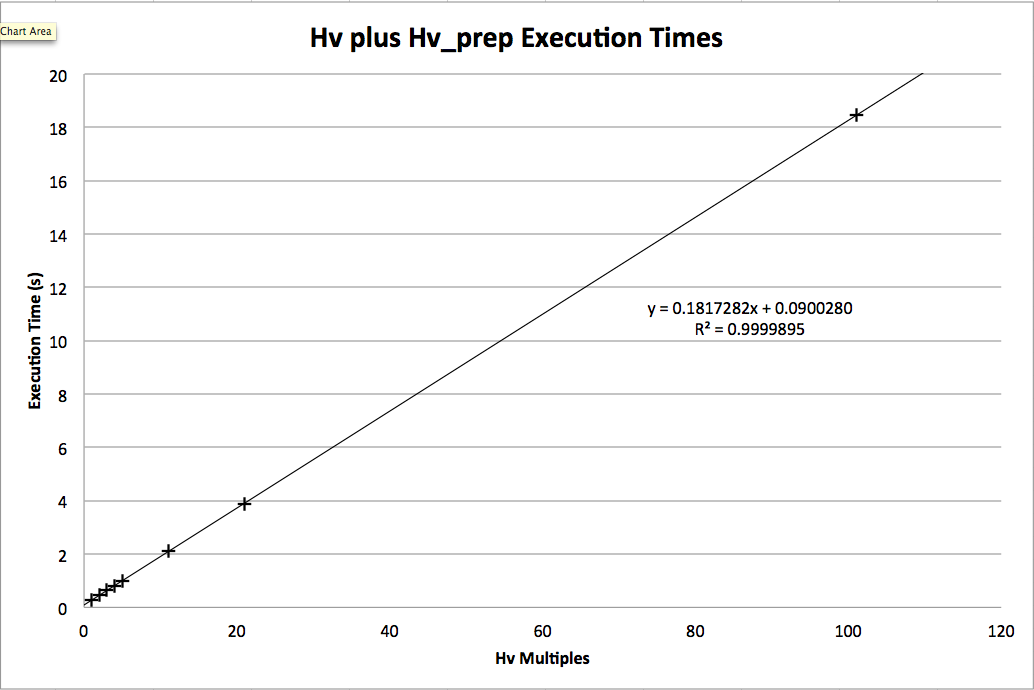
\includegraphics[width=\textwidth,keepaspectratio]{../../Hv-calculators/linRotor/cartSphBasis/Hv-calc/HvHv_prepTimeGraph.png}
\caption{Hv Plus Hv\_Prep Wall Time}
\label{Fig:HvHvPrepExecTime}
\end{figure}


\end{document}